%%%%%%%%%%%%%%%%%%%%%%%%%%%%%%%%%%%%%%%%%%%%%%%%%%%%%%%%%%%%%%%%%%%%%%%%%
\begin{table*}[htb]
\begin{center}
\caption{
Overall results considering relevant information of the best found architectures, detection accuracy (ACC) and HTER values according to the evaluation protocol, and state-of-the-art (SOTA) performance.
}
\label{tab:resultsOARF}
%\tiny  \scriptsize \footnotesize \small \normalsize     
\iffinal
%\small
\else
\scriptsize
\fi
%               MD--TIME---ML--FEAT---L AH AH
\begin{tabular}{llr@{}c@{}l@{ }c@{ }c@{ }r@{ }c@{}l@{ }ccc@{ }ccc@{ }c@{ }c@{}c}
\hline
\multirow{3}{*}{modality}
& \multirow{3}{*}{benchmark} 
                & \multicolumn{9}{c}{architecture optimization (AO)}                     && \multicolumn{2}{c}{our results} && \multicolumn{3}{c}{SOTA results} & \\
                \cline{3-11} 
                \cline{13-14} \cline{16-18} 
&               &  \multicolumn{3}{c}{time}
                           & size 
                                 & layers
                                     & \multicolumn{3}{c}{features} 
                                                                         & objective 
                                                                                  && ACC & HTER && ACC & HTER & \multirow{2}{*}{Ref.}\\
&               & \multicolumn{3}{c}{(secs.)}
                          & (pixels) 
                                 &$(\#)$
                                     & \multicolumn{3}{c}{$(\#)$} 
                                                                          &  $(\%)$    &&$(\%)$ &$(\%)$ &&$(\%)$  & $(\%)$ & \\
\hline\hline
\multirow{2}{*}{iris}
& Warsaw            &  52&+&35 & 640 & 2 & $10\times 15\times  64$ &&  (9600) & 98.21 && \textbf{99.84}
                                                                                            &  0.16 && 97.50  & ---    & \cite{Czajka:MMAR:2013} \\ % *0.0/5.0 MMAR 2013, LivDet'2013 - Iris competion - *5.25%/11.95%  
& Biosec        &  80&+&34 & 640 & 3 & $ 2\times  5\times 256$ &&  (2560) & 97.56 &&  98.93 &  1.17 && \textbf{100.00}
                                                                                                              & ---    & \cite{Galbally:ICB:2012} \\ % ICB 2012 / VISAPP  - IJCANN Porto (99.63%)   
& MobBIOfake    &  18&+&37 & 250 & 2 & $ 5\times  7\times 256$ &&  (8960) & 98.94 &&  98.63 &  1.38 && \textbf{99.75}
                                                                                                                       & ---    & \cite{Sequeira:IJCB:2014} \\ % $0.5/0.0 - MobILive 2014 Competition    
\hline                                      
\multirow{2}{*}{face}
& Replay-Attack &  69&+&15 & 256 & 2 & $ 3\times  3\times 256$ &&  (2304) & 94.65 &&  98.75 &  \textbf{0.75} && ---    &   5.11 & \cite{Komulainen:ICB:2013} \\ %Competition ICB'2013  9.12%   -   0.00%       
& 3DMAD         &  55&+&15 & 128 & 2 & $ 5\times  5\times  64$ &&  (1600) & 98.68 && 100.00 &  \textbf{0.00}
                                                                                                    && ---    &   0.95 & \cite{Erdogmus:BIOSIG:2013}\\ 
\hline
\multirow{2}{*}{fingerprint}
& Biometrika    &  66&+&25 & 256 & 2 & $ 2\times  2\times 256$ &&  (1024) & 90.11 &&  96.50 &  3.50 &&  \textbf{98.30}
                                                                                                                       & ---    & \cite{Ghiani:ICB:2013} \\ % LivDet'2013 - Dermalog     
& Crossmatch    & 112&+&12 & 675 & 3 & $ 2\times  3\times 256$ &&  (1536) & 91.70 && \textbf{92.09} 
                                                                                            &  8.44 &&  68.80 & ---    & \cite{Ghiani:ICB:2013} \\ % LivDet'2013 - UniNap1  
& Italdata      &  46&+&27 & 432 & 3 & $16\times 13\times 128$ && (26624) & 86.89 &&  97.45 &  2.55 &&  \textbf{99.40}
                                                                                                                       & ---    & \cite{Ghiani:ICB:2013} \\ % LivDet'2013 - Anonymous2   
& Swipe         &  97&+&51 & 962 & 2 & $53\times  3\times  32$ &&  (5088) & 90.32 &&  88.94 & 11.47 &&  \textbf{96.47}
                                                                                                                       & ---    & \cite{Ghiani:ICB:2013} \\ % LivDet'2013 - Dermalog     
\hline
\end{tabular}
\end{center}
\end{table*}
%%%%%%%%%%%%%%%%%%%%%%%%%%%%%%%%%%%%%%%%%%%%%%%%%%%%%%%%%%%%%%%%%%%%%%%%%%%

\section{Experiments and Results}
\label{sec:experiments}



In this section, we evaluate the effectiveness of the proposed methods for spoofing detection. We show experiments for the architecture optimization and filter learning approaches along with their combination  
for detecting iris, face, and fingerprint spoofing on the nine benchmarks described in Section~\ref{sec:databases}. We also present results for the \emph{spoofnet}, which incorporates some domain-knowledge on the problem. We compare all of the results with the state-of-the-art counterparts. Finally, we discuss the pros and cons of using such approaches and their combination along with efforts to understand the type of features learned and some effeciency questions when testing the proposed methods.



\subsection{Architecture Optimization (AO)}

Table~\ref{tab:resultsOARF} presents AO results in detail as well as previous state-of-the-art (SOTA) performance for the considered benchmarks. With this approach, we can outperform four SOTA methods in all three biometric modalities. Given that AO assumes little knowledge about the problem domain, this is remarkable. Moreover, performance is on par in other four benchmarks, with the only exception of Swipe. Still in Table~\ref{tab:resultsOARF}, we can see information about the best architecture such as time taken to evaluate it (feature extraction + 10-fold validation), input size, depth, and dimensionality of the output representation in terms of \emph{columns} $\times$ \emph{rows} $\times$ \emph{feature maps}.

Regarding the number of layers in the best architectures, we can observe that six out of nine networks use two layers, and three use three layers. We speculate that the number of layers obtained is a function of the problem complexity.
In fact, even though there are many other hyperparameters involved, the number of layers play an important role in this issue, since it directly influences the level of non-linearity and abstraction of the output with respect to the input.

With respect to the input size, we can see in comparison with Table~\ref{tab:databases:experiments}, that the best performing architectures often use the original image size. This was the case for all iris benchmarks and for three (out of four) fingerprint benchmarks. For face benchmarks, a larger input was preferred for Replay-Attack, while a smaller input was preferred for 3DMAD. We hypothesize that this is also related to the problem difficulty, given that Replay-Attack seems to be more difficult, and that larger inputs tend to lead to larger networks.

We still notice that the dimensionality of the obtained representations are, in general, smaller than 10K features, except for Italdata.
Moreover, for the face and iris benchmarks, it is possible to roughly observe a relationship between the optimization objective calculated in the training set and the detection accuracy measure on the testing set (Section~\ref{sec:evalprot}), which indicates the appropriateness of the objective for these tasks. However, for the fingerprint benchmarks, this relationship does not exist, and we accredit this to either a deficiency of the optimization objective in modelling these problems or to the existence of artifacts in the training set misguiding the optimization.

% Table~\ref{tab:resultsOARF} shows the overall results and is divided in three parts.
% We can see that the performance of proposed methods are competitive. In fact, by training simple linear classifiers on the deep representations found with the architecture optimization approach, the proposed methods outperform four SOTA methods and are on par with other four methods. 
% In particular, we obtained state-of-the-art performance on the Warsaw (iris), Replay-Attack (face), 3DMAD (face), and CrossMatch (fingerprint) benchmarks, at least one in each biometric modality. When considering architecture optimization, the less compelling result was for the Swipe benchmark.

% Analysing the first part of Table~\ref{tab:resultsOARF}, we can observe important characteristics of the best CNNs found in the architecture hyperparameter optimization step such as the time (in seconds) taken to evaluate it (feature extraction + 10-run validation), the input size that the CNN assumes ($\max_{axis}$), its depth ($d_{choice}$), and the dimensionality of its output representations in terms of \emph{columns} $\times$ \emph{rows} $\times$ \emph{bands}.

% Taking into account that understanding how a set of deep learned features capture properties and nuances of a problem is still an open question in the vision community, in the following we discuss the listed properties of the optimized CNNs that may bring clues and insights on how these features are meaningful for the spoofing problem.

% Regarding the number of layers required by the CNNs producing the best representations, we can observe that six out of nine CNNs use two layers, and three CNNs use three layers.
% We speculate that the number of layers obtained is a function of the problem complexity.
% Even though there are many other hyperparameters involved, the number of layers play an important role in this issue, since it directly influences the level of non-linearity and abstraction of the output with respect to the input.

% \TODO{This is still true? Before you mentioned for the spoofnet that wanted larger images as a domain-knowledge to incorporate more information. This is not in line with that}
% Regarding input image size ($\max_{axis}$), in comparison with Table~\ref{tab:databases:experiments}, we can see that the best performing CNNs often use the original image size. This was the case for all iris benchmarks and for three (out of four) fingerprint benchmarks. For the face benchmarks, a larger input was preferred for Replay-Attack, while a smaller input was preferred for 3DMAD. We hypothesize that this is also related to the problem difficulty, given that Replay-Attack seems to be more difficult, and that larger inputs tend to lead to larger networks.

% Still with respect to the outcomes of the optimization, we notice that the dimensionality of the obtained representations are, in general, smaller than 10K features, except for Italdata.
% Moreover, for the face and iris benchmarks, it is possible to roughly observe a relationship between the optimization objective calculated in the training set and the detection accuracy measure on the testing set (Section~\ref{sec:evalprot}), which indicates the appropriateness of the objective for these tasks. However, for the fingerprint benchmarks, this relationship does not exists, and we accredit this to either a deficiency of the optimization objective in modeling these problems or the existence of artifacts in the training set misguiding the optimization.


\subsection{Filter Optimization (FO)}

\begin{table}
\begin{center}
\caption{
Results for filter optimization (FO) in \emph{cf10-11} and \emph{spoofnet} (Fig.~\ref{fig:cudaconvnet}). Even though both networks present similar behavior, \emph{spoofnet} is able to push performance even further in problems which \emph{cf10-11} was already good for.
Architecture optimization (AO) results (with random filters) are shown in the first column to facilitate comparisons.
}
\label{tab:FO}
\begin{tabular}{c@{ }c@{ }l@{ }r@{ }r@{ }r@{ }r@{ }r@{ }r@{ }r@{ }r@{ }c}
\hline
% \multirow{2}{*}{benchmark} 
         & \hspace{1em} && \multicolumn{6}{c}{filter}\\ \cline{4-9}
modality & \hspace{1em} &&& random && \multicolumn{3}{c}{optimized} \\ \cline{5-5} \cline{7-9}
(metric) && benchmark \hspace{1em} && \multicolumn{1}{c}{AO} && \textit{cf10-11} && \textit{spoofnet} && SOTA & \\
\hline
iris && Warsaw        && \textbf{99.84}  && 67.20 &&          66.42  &&          97.50 \\
(ACC)&& Biosec        &&         98.93   && 59.08 &&          47.67  && \textbf{100.00} \\
     && MobBIOfake    &&         98.63   && 99.13 && \textbf{100.00} &&          99.75 \\
\hline
face && Replay-Attack &&\textbf{0.75} && 55.13 && 55.38 && 5.11\\
(HTER) && 3DMAD         &&\textbf{0.00} && 40.00 && 24.00 && 0.95\\ 
\hline
fingerprint &&Biometrika    && 96.50 && 98.50&& \textbf{99.85} && 98.30\\
(ACC)     &&Crossmatch    && 92.09 && 97.33&& \textbf{98.23} && 68.80\\
     &&Italdata      && 97.45 && 97.35&& \textbf{99.95} && 99.40\\
     &&Swipe         && 88.94 && 98.70&& \textbf{99.08} && 96.47\\
\hline
\end{tabular}
\end{center}
\end{table}

% \begin{table}
% \red{
% \begin{center}
% \caption{\TODO{write me}}
% \label{tab:FO}
% \begin{tabular}{l@{ }c@{ }c@{ }c@{ }c@{ }c@{ }c@{ }c@{ }c@{ }c@{ }c@{ }c@{ }c}
% \hline
% \multirow{2}{*}{benchmark} 
%                 && \multicolumn{2}{c}{OA} && \multicolumn{2}{c}{\textit{cf10-11}} && \multicolumn{2}{c}{\textit{spoofnet}} && SOTA & \\
%                 \cline{3-4} \cline{6-7} \cline{9-10} 
%                 \cline{12-12}
%                &&$(\%)$&$(\%)$&&$(\%)$&$(\%)$&&$(\%)$&$(\%)$&&$(\%)$\\
% \hline\hline
% Warsaw        && \textbf{99.84}  & 59.55 && 87.06 & 67.20 && 96.44 &          66.42  &&          97.50 \\
% Biosec        &&         98.93   & 57.50 && 97.33 & 59.08 && 97.42 &          47.67  && \textbf{100.00} \\
% MobBIOfake    &&         98.63   & 99.38 && 77.00 & 99.13 && 72.00 & \textbf{100.00} &&          99.75 \\
% \hline
% Replay-Attack &&\textit{\textbf{0.75}} & \textit{55.88} &&\textit{5.62} &\textit{55.13} &&\textit{3.50} &\textit{55.38} &&\textit{5.11}\\
% 3DMAD         &&\textit{\textbf{0.00}} & \textit{40.00} &&\textit{8.00} &\textit{ 40.00}&&\textit{4.00} &\textit{ 24.00}&&\textit{0.95}\\ 
% \hline
% Biometrika    && 96.50& 99.30&& 77.45& 98.50&& 94.70&\textbf{99.85} && 98.30\\
% Crossmatch    && 92.09& 98.04&& 83.11& 97.33&& 87.82&\textbf{98.23} && 68.80\\
% Italdata      && 97.45& 99.45&& 76.45& 97.35&& 91.05&\textbf{99.95} && 99.40\\
% Swipe         && 88.94& 99.08&& 87.60& 98.70&& 96.75&\textbf{99.08} && 96.47\\
% \hline
% \end{tabular}
% \end{center}
% Abbreviations: \emph{OA} - Optimized Architecture; \emph{Arc.} - Architecture; \emph{RF} - random filters; \emph{LF} - learned filter through backpropagation
% }
% \end{table}


Table~\ref{tab:FO} shows the results for FO, where we repeat architecture optimization (AO) results (with random filters) in the first column to facilitate comparisons. Overall, we can see that both networks, \emph{cf10-11} and \emph{spoofnet} have similar behavior across the biometric modalities.

Surprisingly, \emph{cf10-11} obtains excellent performance in all four fingerprint benchmarks as well as in the MobBIOFake, exceeding SOTA in three cases, in spite of the fact that it was used without any modification. However, in both face problems and in two iris problems, \emph{cf10-11} performed poorly. Such difference in performance was not possible to anticipate by observing training errors, which steadily decreased in all cases until training was stopped. Therefore, we believe that in these cases FO was misguided by the lack of training data or structure in the training samples irrelevant to the problem.
% Even though they perform both poorly in Warsaw, Biosec, Replay-Attack and 3DMAD, they

%% THIS PART BELOW GOES TO THE TEXT AFTER THE SSS CLAIM
\rva{To reinforce this claim, we performed experiments with filter optimization (FO) in \emph{spoofnet} by varying the training set size with 20\%, 40\%, and 50\% of fingerprint benchmarks. As expected, in all cases, the less training examples, the worse is the generalization of the \emph{spoofnet} (lower classification accuracies). 
Considering the training phase, for instance, when using 50\% of training set or less, the accuracy achieved by the learned representation is far worse than the one achieved when using 100\% of training data. 
This fact reinforces the conclusion presented herein regarding the small sample size problem. 
Maybe a fine-tuning of some parameters, such as the number of training epochs and the learning rates, can diminish the impact of the small sample size problem stated here, however, this is an open research topic by itself.}

For \emph{spoofnet}, the outcome is similar. As we expected, the proposed architecture was able to push performance even further in problems which \emph{cf10-11} was already good for, outperforming SOTA in five out of nine benchmarks. This is possibly because we made the \emph{spoofnet} architecture simpler, with less parameters, and taking input images with a size better suited to the problem.

As compared to the results in AO, we can observe a good balance between the approaches. In AO, the resulting convolutional networks are remarkable in the face benchmarks. In FO, networks are remarkable in fingerprint problems. While in AO all optimized architectures have good performance in iris problems, FO excelled in one of these problems, MobBIOFake, with a classification accuracy of 100\%. In general, AO seems to result in convolutional networks that are more stable across the benchmarks, while FO shines in problems in which learning effectively occurs. Considering both AO and FO, we can see in Table~\ref{tab:FO} that we outperformed SOTA methods in eight out of nine benchmarks. The only benchmark were SOTA performance was not achieved is Biosec, but even in this case the result obtained with AO is competitive. 

%%\TODO{Allan's figure discussion starts here.}
%\input{fig_allan}
Understanding how a set of deep learned features capture properties and nuances of a problem is still an open question in the vision community. However, in an attempt to understand the behavior of the operations applied onto images after they are forwarded through the first convolutional layer, we generate Fig.~\ref{fig:filter_learned_conv1} that illustrates the filters learned via backpropagation algorithm and Figs.~\ref{fig:mean_pos_class}~and~\ref{fig:mean_neg_class} showing the mean of real and fake images that compose the test set, respectively. To obtain output values from the first convolutional layer and get a sense of them, we also instrumented the \textit{spoofnet} convolutional network to forward the real and fake images from the test set through network. Figs~\ref{fig:act_map_class_1}~and~\ref{fig:act_map_class_0} show such images for the real and fake classes, respectively.

We can see in Fig.~\ref{fig:filter_learned_conv1} that the filters learned patterns resemble textural patterns instead of edge patterns as usually occurs in several computer vision problems~\cite{Krizhevsky:2012,Ouyang:2014}. This is particularly interesting and in line with several anti-spoofing methods in the the literature which also report good results when exploring texture information~\cite{Ghiani:ICB:2013, Maatta:IJCB:2011}.

In addition, Fig.~\ref{fig:mean_pos_class}~and~\ref{fig:mean_neg_class} show there are differences between real and fake images from test, although apparently small in such a way that a direct analysis of the images would not be enough for decision making. However, when we analyze the mean activation maps for each class, we can see more interesting patterns. In Figs.~\ref{fig:act_map_class_1}~and~\ref{fig:act_map_class_0}, we have sixteen pictures with $128 \times 128$ pixel resolution. These images correspond to the sixteen filters that composing the first layer of the \textit{spoofnet}. Each position $(x,y)$ in these $128 \times 128$ images corresponds to a $5 \times 5$ area (receptive field units) in the input images. Null values in a given unit means that the receptive field of the unit was not able to respond to the input stimuli. In contrast, non-null values mean that the receptive field of the unit had a responsiveness to the input stimuli.

We can see that six filters have a high responsiveness to the background information of the input images (filters predominantly white) whilst ten filters did not respond to background information (filters predominantly black). From left to right, top to bottom, we can see  also that the images corresponding to the filters 2, 7, 13, 14 and 15 have high responsiveness to information surrounding the central region of the sensor (usually where fingerprints are present) and rich in texture datails. Although these regions of high and low responsiveness are similar for both classes we can notice some differences. A significant difference in this first convolutional layer to images for the different classes is that the response of the filters regarding to fake images (Fig~\ref{fig:act_map_class_0}) generates a blurring pattern, unlike the responses of the filters regarding to real images (Fig~\ref{fig:act_map_class_1}) which generate a sharper pattern. We believe that the same way as the first layer of a convolutional network has the ability to respond to simple and relevant patterns (edge information) to a problem of recognition objects in general, in computer vision, the first layer in the \textit{spoofnet} also was able to react to a simple pattern recurrent in spoof problems, the blurring effect, an artifact previously explored in the literature~\cite{Galbally:TIP:2014}. Finally, we are exploring visualisation only of the first layer; subsequent layers of the network can find new patterns in these regions activated by the first layer further emphasizing class differences. 

\begin{figure}
\centering
\subfloat[Filter weights of the first convolutional layer that were learned using the backpropagation algorithm.]{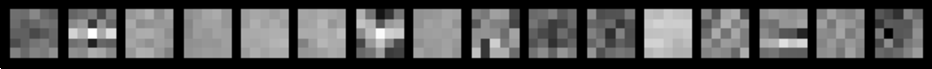
\includegraphics[width=0.46\textwidth]{crossmatch_conv1_without_background.pdf}\label{fig:filter_learned_conv1}}\\
\subfloat[Mean for real images (test set).]{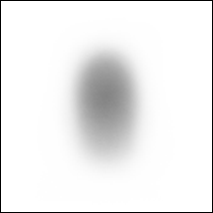
\includegraphics[width=0.20\textwidth]{crossmatch_test_pos_class_with_border.pdf}\label{fig:mean_pos_class}}\hspace{1mm}
\subfloat[Mean for fake images (test set).]{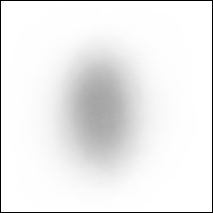
\includegraphics[width=0.20\textwidth]{crossmatch_test_neg_class_with_border.pdf}\label{fig:mean_neg_class}}\\
\subfloat[Activation maps for real images.]{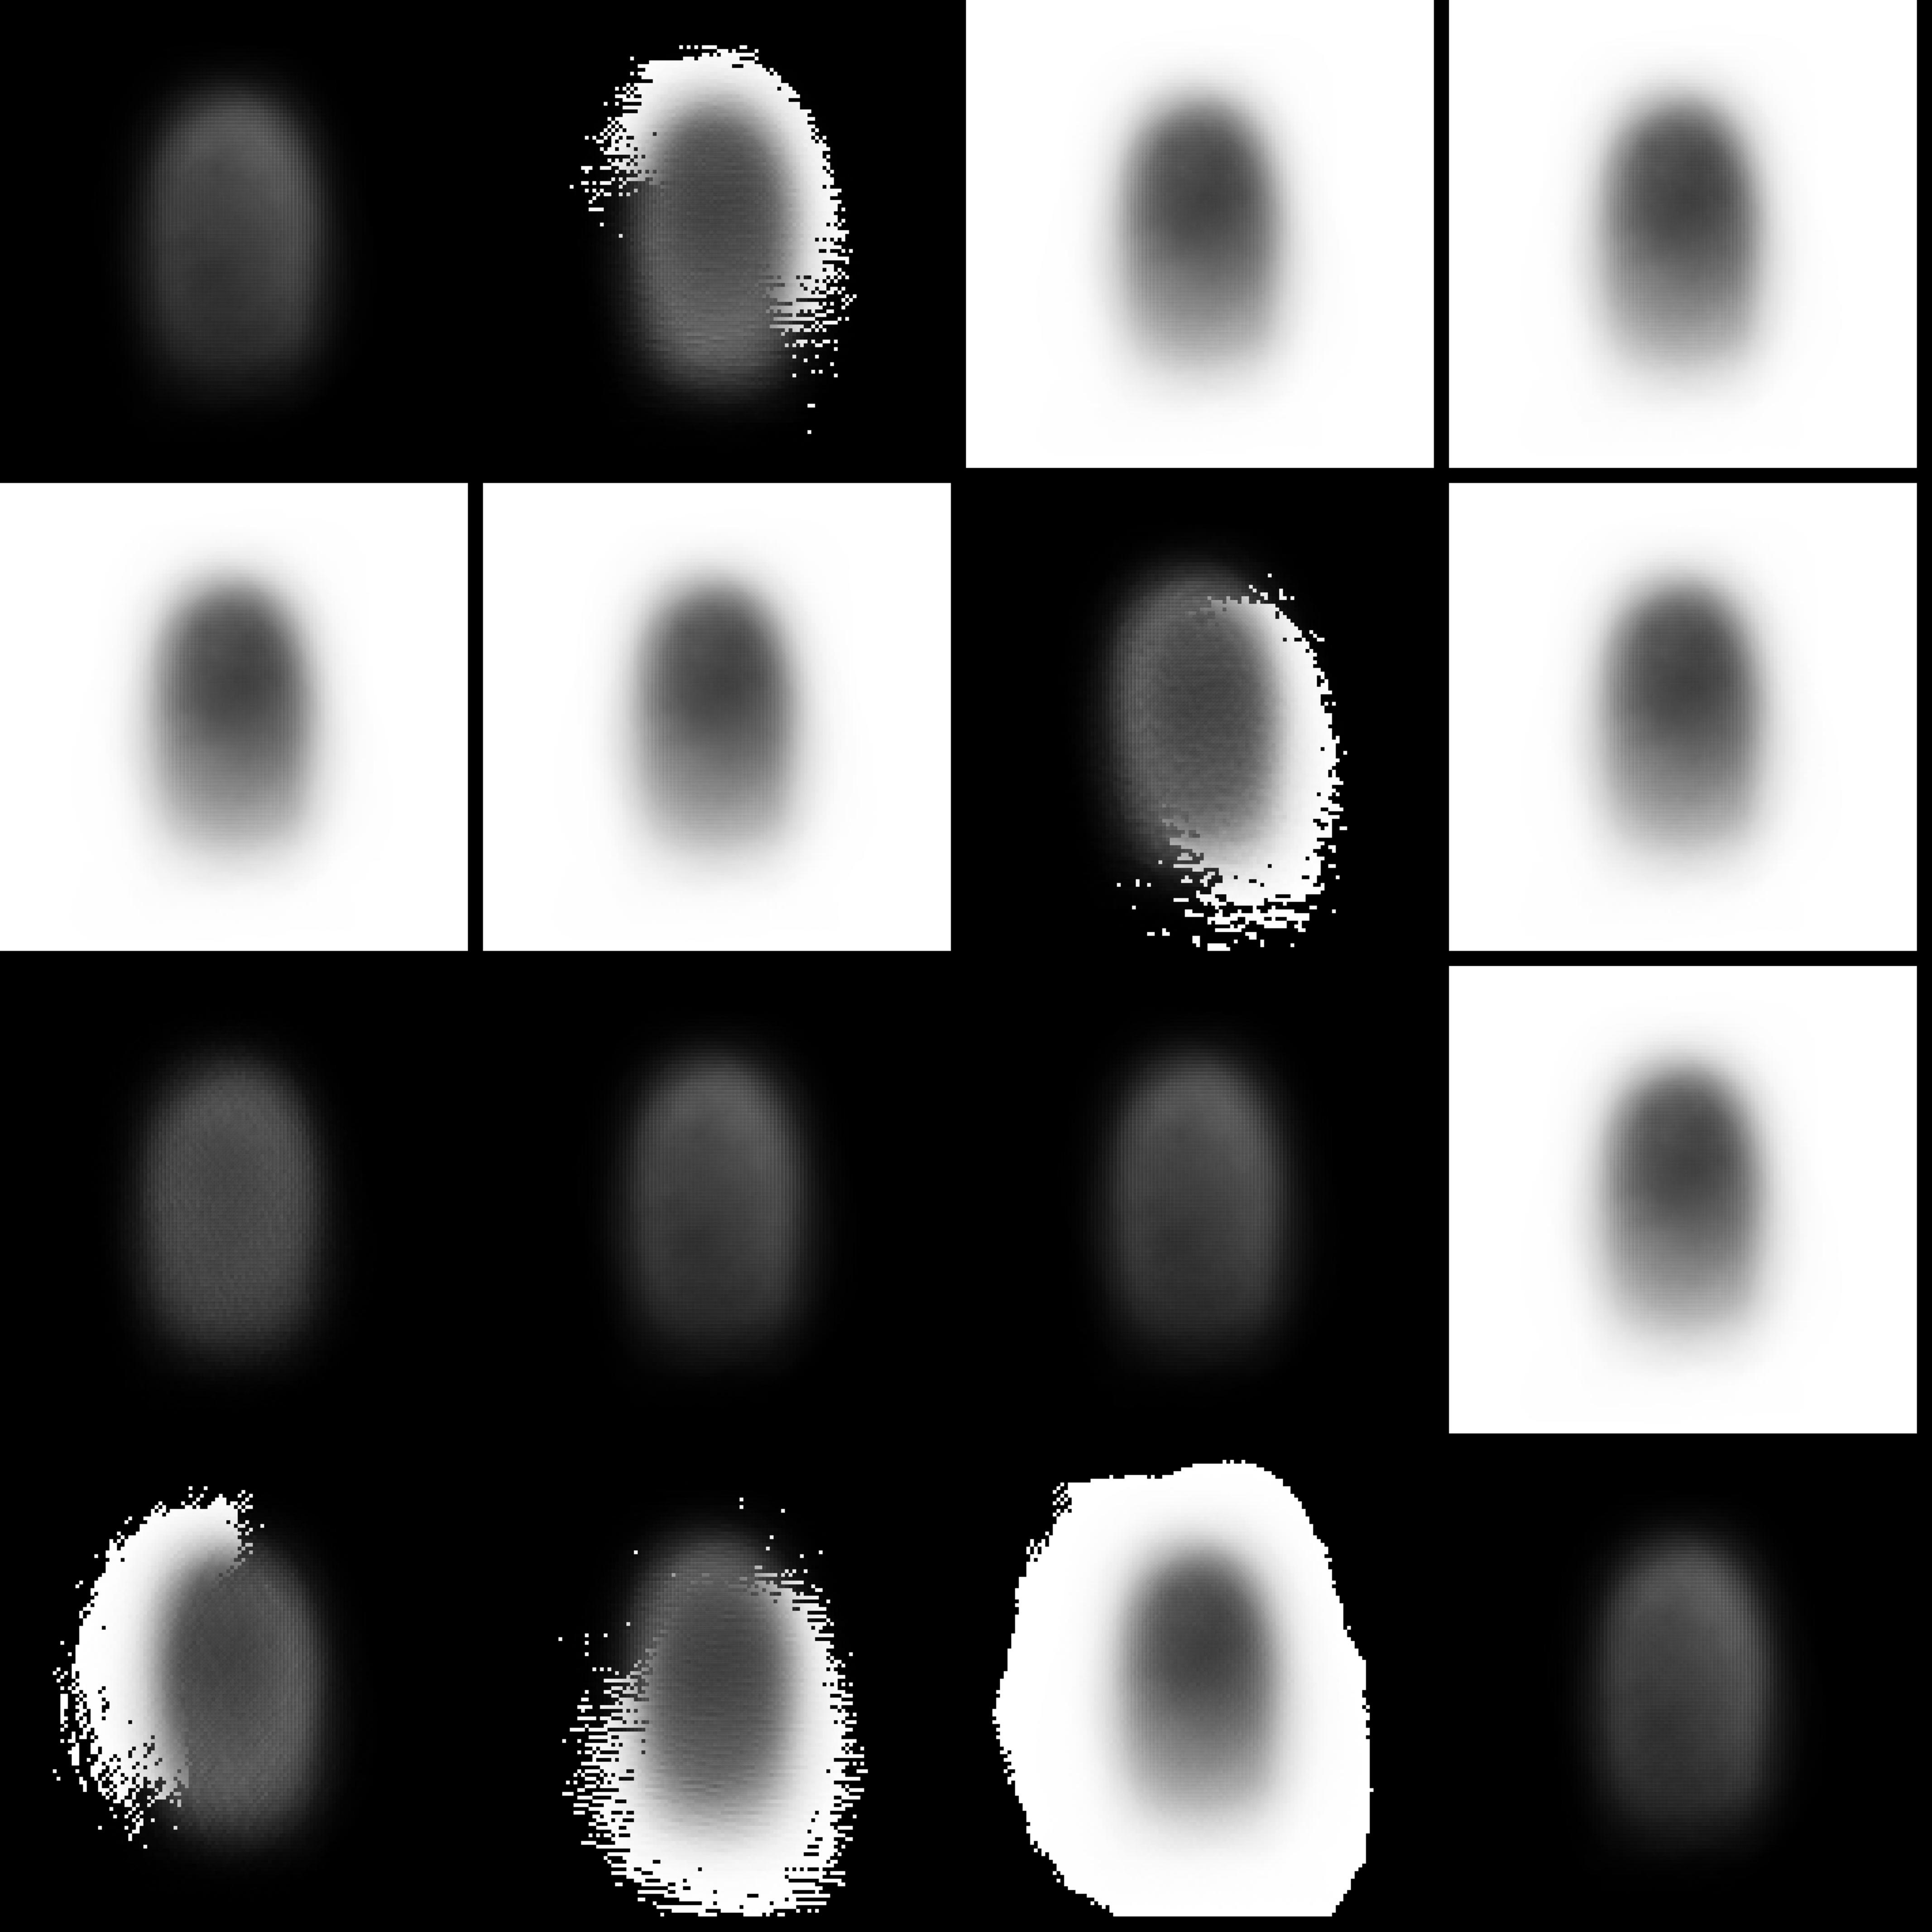
\includegraphics[width=0.23\textwidth]{crossmatch_activation_map_class_1.pdf}\label{fig:act_map_class_1}}\hspace{1mm}
\subfloat[Activation maps for fake images.]{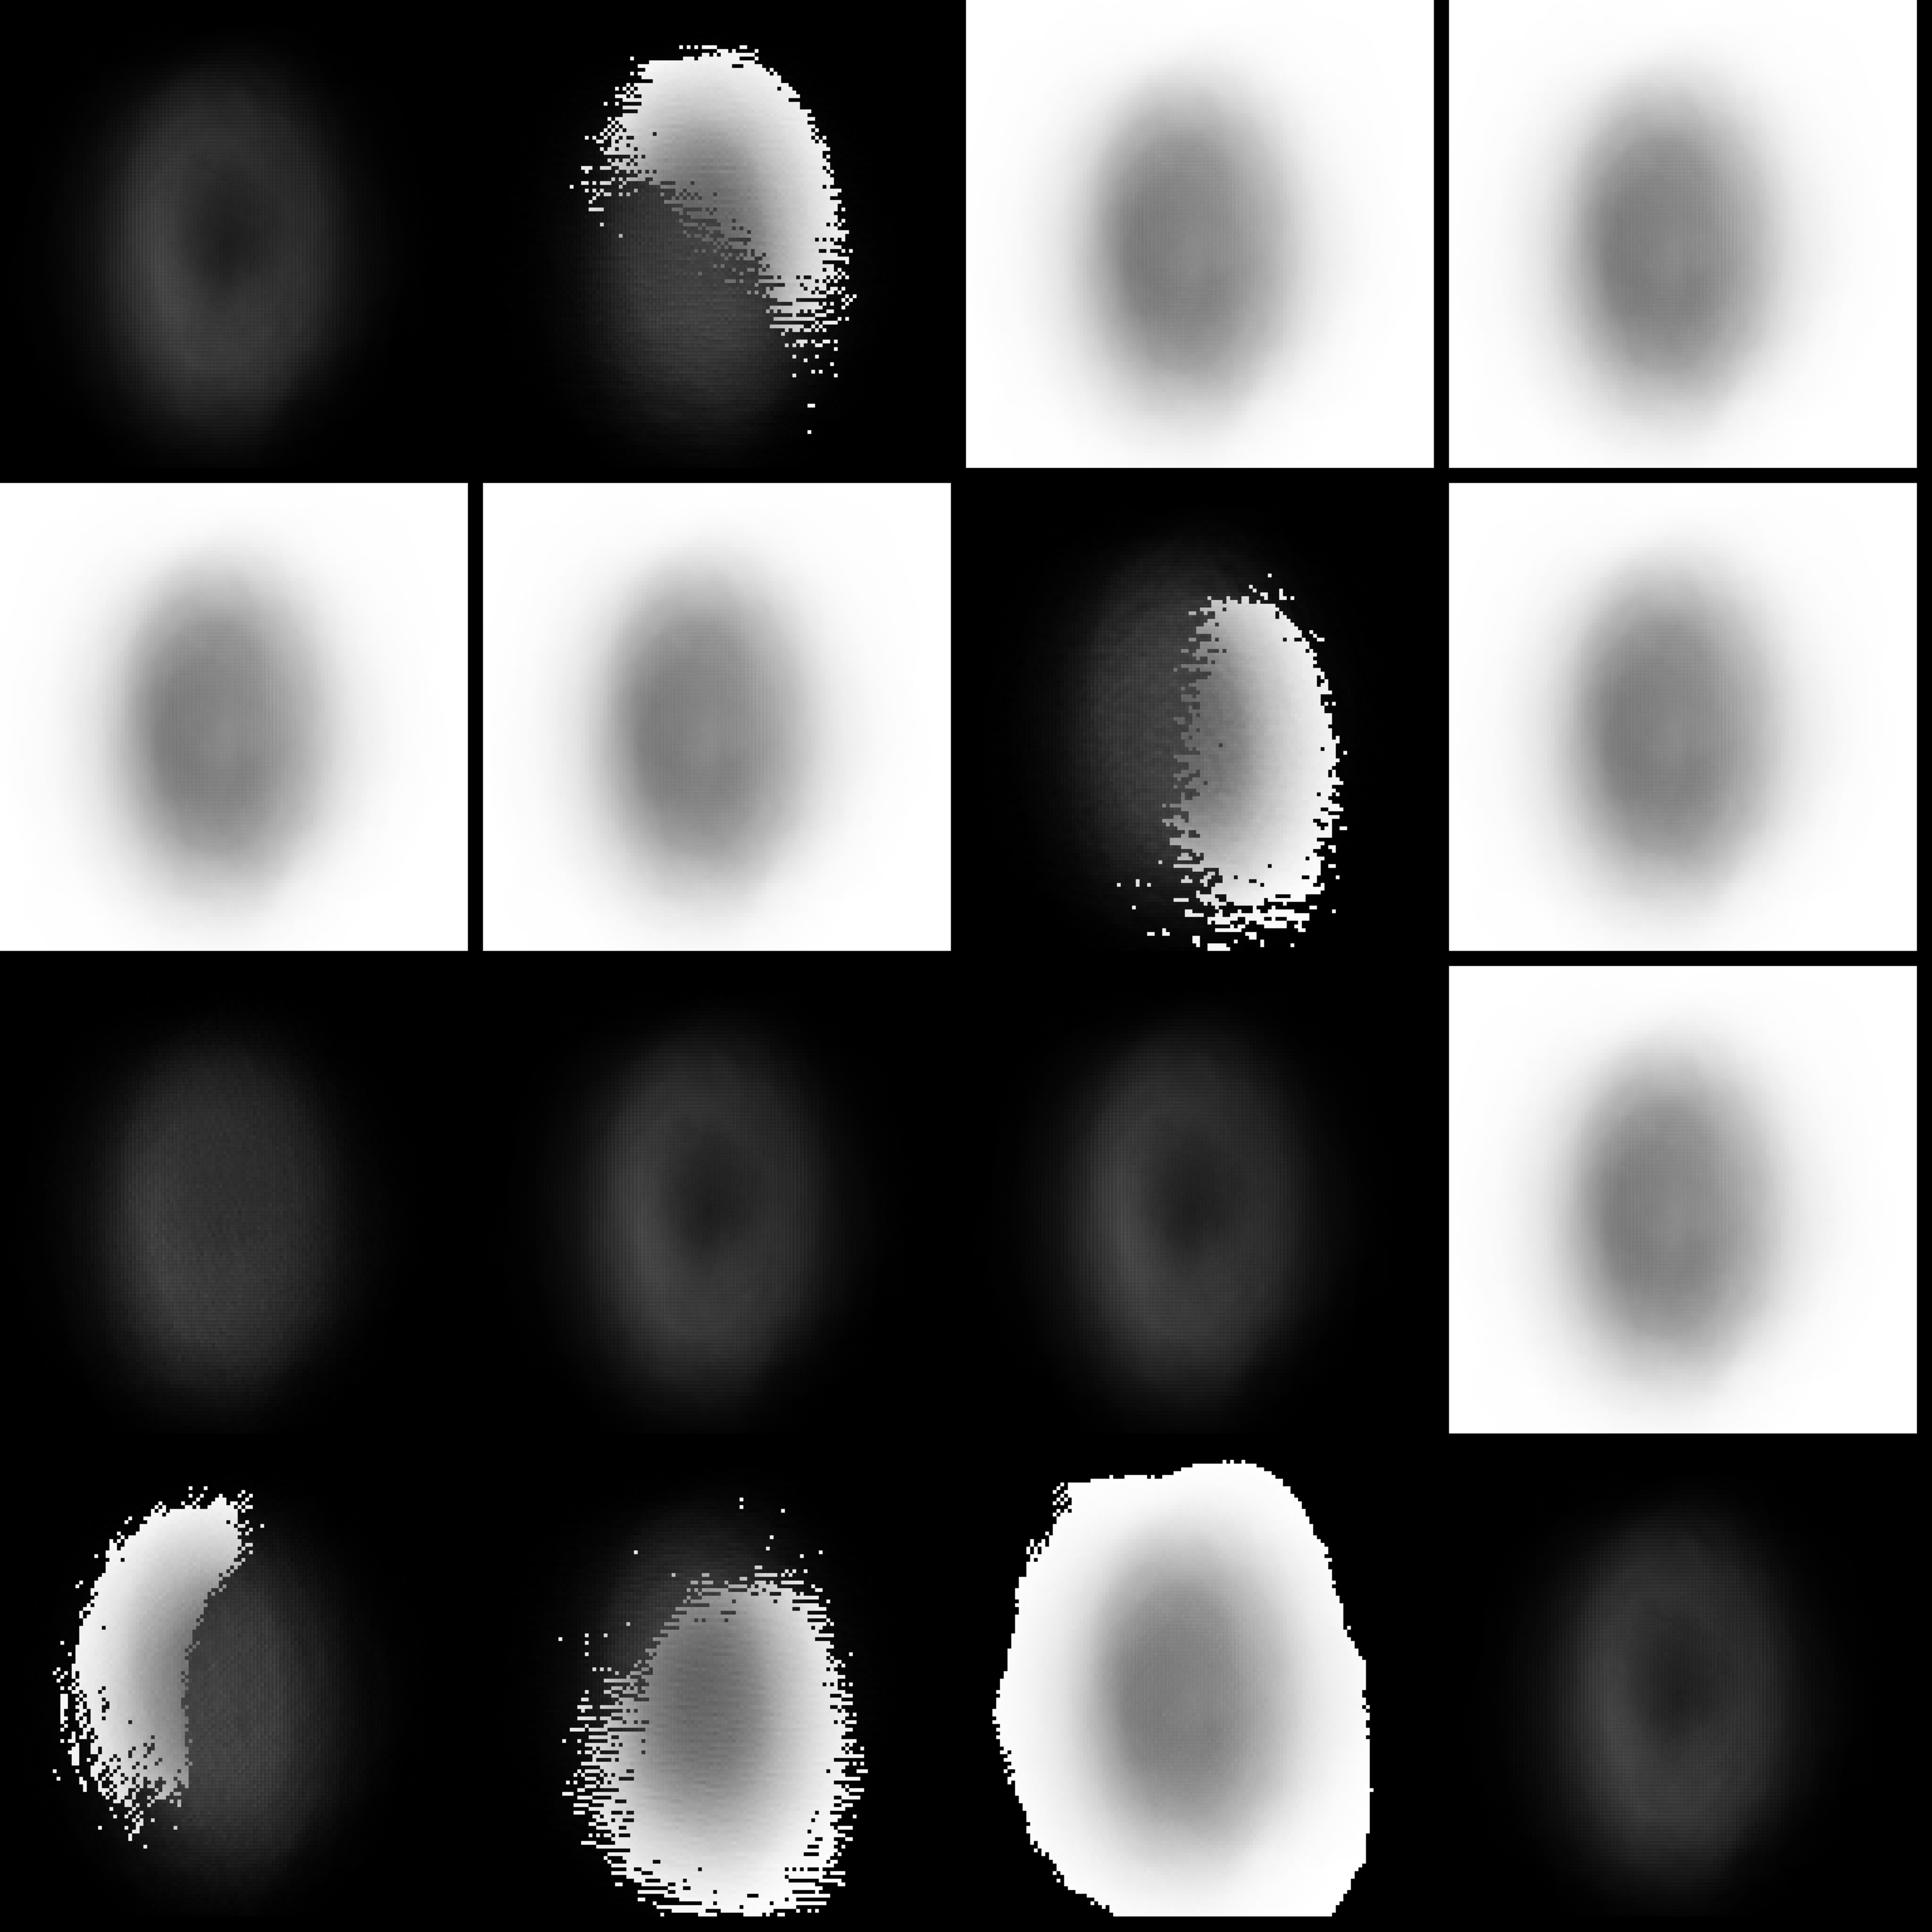
\includegraphics[width=0.23\textwidth]{crossmatch_activation_map_class_0.pdf}\label{fig:act_map_class_0}}\\

\caption{Activation maps of the filters that compose the first convolutional layer when forwarding real and fake images through the network.}
\end{figure}

% The last round of experiments evaluates the \emph{spoofnet} architecture, which incorporates our domain-knowledge on the problem taken from observations of the architecture optimization experience.
% That is, given that we are working on a relatively simple and binary problem different from the traditional multiclass problems present in vision, a small and less complex network could be able to accommodate the variability of the spoofing problem more effectively.
% Moreover, the use of a large input image could also be beneficial to obtain better features of the recapture process inherent to spoofing such as the ones related to the added noise signatures during the process.
% We compare such network considering random and learned filter weights and show results on Table~\ref{tab:compAll}.

% In this scenario, the \textit{spoofnet} has systematically outperformed \textit{cf10-11}'s network and the optimized architecture in the benchmarks for which filter learning approach performed well in previous experiments.

% Moreover, \textit{spoofnet} outperforms the SOTA results in five out nine  benchmarks, and the architecture optimization approach outperforms the SOTA results in another three benchmarks.

% That is, the combination of the proposed methods achieves new SOTA results in eight out nine cases, three SOTA results when optimizing the architecture and using random filters and five SOTA results when incorporating domain-knowledge in the design of a network using learned filters.
% The only case in which the use of convolutional networks as proposed here does not achieve SOTA results is for the Biosec benchmark. 
% In this case, the proposed method using architecture optimization provides a result of about 1\% lower than the SOTA, which is still a remarkable accomplishment (98.93\% v. 100.0\% classification accuracy).

% The final remark is that the filter learning approach has always failed to four benchmarks: Warsaw, Biosec, Replay-Attack, and 3DMAD.
% Our hypotheses for such fact are threefold:  
% (1) the existence of few samples available, which hinders the learning process;  
% (2) the lack of variability (subjects, sessions, etc.) in the training set limiting the generalization of the learned representation; and 
% (3) particular nuances existing in the testing set not present in the training set (e.g., due to different session acquisition conditions) that could not be captured in the learning process but could be incorporated by the architecture optimization approach.



% Tables~\ref{tab:resultsOARF},~\ref{tab:compOAAA}, and~\ref{tab:compAll} present the effectiveness results for spoofing detection considering the proposed methods with respect to the state of the art. 
% In Tables~\ref{tab:compOAAA} and~\ref{tab:compAll} we present the accuracy values, except when they are in \emph{italic}. When in italic, the value refers to HTER values, the standard evaluation measure for Replay-Attack and 3DMAD benchmarks.

% We now turn our attention to our second set of contributions, more specifically, when considering an approach for learning filter weights on a given network. Given a well-known architecture in a given scenario (e.g., vision problems), such as \textit{cf10-11}, we learn its filter weights using the methodology described in Section~\ref{sec:fwl_training}.
% Then, we compare their effectiveness with the ones of the architecture optimization.

% Two important aspects can be observed here. First, the filter learning approach (\textit{cf10-11}+LF) outperforms the existing SOTA results on three out of nine benchmarks, that is, Biometrika, Crossmatch and Swipe -- all fingerprint benchmarks. It also outperforms the architecture optimization approach (OA+RF) on another benchmark, MobBIOfake (iris).
% The effectiveness achieved by the filter learning approach (\textit{cf10-11}+LF) in four benchmarks (Warsaw, Biosec, Replay-Attack and 3DMAD), on the other hand, might be surprising as the network here was learned for a vision problem and only its filters were learned for spoofing problems.


\subsection{Interplay between AO and FO}

\begin{table}
\begin{center}
\caption{Results for architecture and filter optimization (AO+FO) along with \emph{cf10-11} and \emph{spoofnet} networks considering random weights.
AO+FO show compelling results for fingerprints and one iris benchmark (MobBIOFake). We can also see that \emph{spoofnet} can benefit from random filters in situations it was not good for when using filter learning (e.g., Replay-Attack).}
\label{tab:interplay}
\begin{tabular}{c@{ }c@{ }l@{ }r@{ }c@{ }r@{ }r@{ }r@{ }r@{ }r@{ }r@{ }c}
\hline
% \multirow{2}{*}{benchmark} 
         & \hspace{1em} && \multicolumn{6}{c}{filter}\\ \cline{4-9}
modality & \hspace{1em} &&& optimized && \multicolumn{3}{c}{random} \\ \cline{5-5} \cline{7-9}
(metric) && benchmark \hspace{1em} && AO && \textit{cf10-11} && \textit{spoofnet} && SOTA & \\
\hline
iris && Warsaw        &&                59.55  && 87.06 &&          96.44  && \textbf{ 97.50} \\
(ACC)&& Biosec        &&                57.50  && 97.33 &&          97.42  && \textbf{100.00} \\
     && MobBIOfake    &&                99.38  && 77.00 &&          72.00  &&  \textbf{ 99.75} \\
\hline
face && Replay-Attack &&                55.88  &&  5.62 &&  \textbf{ 3.50} &&           5.11 \\
(HTER) && 3DMAD       &&                40.00  &&  8.00 &&           4.00  &&  \textbf{ 0.95} \\ 
\hline
fingerprint &&Biometrika     && \textbf{99.30}  && 77.45 &&          94.70  &&           98.30\\
(ACC)     &&Crossmatch       && \textbf{98.04}  && 83.11 &&          87.82  &&           68.80\\
     &&Italdata              && \textbf{99.45}  && 76.45 &&          91.05  &&           99.40\\
     &&Swipe                 && \textbf{99.08}  && 87.60 &&          96.75  &&           96.47\\
\hline
\end{tabular}
\end{center}
\end{table}

In the previous experiments, architecture optimization (AO) was evaluated using random filters and filter optimization (FO) was carried out in the predefined architectures \emph{cf10-11} and \emph{spoofnet}. A natural question that emerges in this context is how these methods would perform if we (i) combine AO and FO and if we (ii) consider random filters in \emph{cf10-11} and \emph{spoofnet}.

Results from these combinations are available in Table~\ref{tab:interplay} and show a clear pattern. When combined with AO, FO again exceeds previous SOTA in all fingerprint benchmarks and performs remarkably good in MobBIOFake. However, the same difficulty found by FO in previous experiments for both face and two iris benchmarks is also observed here.
Even though \emph{spoofnet} performs slightly better than AO in the cases where SOTA is exceeded (Table~\ref{tab:FO}), it is important to remark that our AO approach may result in architectures with a much larger number of filter weights to be optimized, and this may have benefited~\emph{spoofnet}.

It is also interesting to observe in Table~\ref{tab:interplay} the results obtained with the use of random filters in \emph{cf10-11} and \emph{spoofnet}. The overall balance in performance of both networks across the benchmarks is improved, similar to what we have observed with the use of random filters in Table~\ref{tab:resultsOARF}. An striking observation is that~\emph{spoofnet} with random filters exceed previous SOTA in Replay-Attack, and this supports the idea that the poor performance of~\emph{spoofnet} in Replay-Attack observed in the FO experiments (Table~\ref{tab:FO}) was not a matter of architecture.


% Second, the \textit{cf10-11} network when using random filters (\textit{cf10-11}+RF) shows a relatively high effectiveness when compared to the learning filter approach (\textit{cf10-11}+LF) on four datasets where the learning approach clearly fails (Warsaw, Biosec, Replay-Attack, 3DMAD).

% Finally, another interesting observation: the optimized architectures with learned filters (OA+LF) achieved better classification results than the ones of \textit{cf10-11} whenever the \textit{cf10-11}+LF worked well. In such cases, the combination of architecture and filter optimization approaches outperformed the SOTA results in seven out of nine benchmarks.

% The \textit{spoofnet} with random filters has achieved promising results in almost all benchmarks (except for MobBIOfake), and has outperformed the previous SOTA results for the Crossmatch and Swipe benchmarks. That is, if someone does not have enough data or time to train an optimized architecture, this solution be a good tradeoff. 


% \begin{table}[htb]
% \red{
% \begin{center}
% \caption{The effects of combining existing (cf10-11) and optimized architectures (OA) with filter learning (LF) and random filters (RF).}
% \label{tab:compOAAA}
% %\tiny  \scriptsize \footnotesize \small \normalsize     
% \iffinal
% %\small
% \else
% \scriptsize
% \fi
% %               MD--TIME---ML--FEAT---L AH AH
% \begin{tabular}{l@{ }c@{ }c@{ }c@{ }c@{ }c@{ }c@{ }c@{ }c@{ }c}
% \hline
% \multirow{3}{*}{Database} 
%                 && \multicolumn{2}{c}{OA} 
%                                                       && \multicolumn{2}{c}{\textit{cf10-11}} 
%                                                                                            && SOTA & \\
                
%                 \cline{3-4} \cline{6-7} 
%                && RF & LF && RF & LF && Results & \\
%                                                                \cline{9-9}      
%                &&$(\%)$&$(\%)$&&$(\%)$&$(\%)$&&$(\%)$\\
% \hline\hline
% Warsaw        && \textbf{99.84} 
%                       & 59.55&& 87.06& 67.20&& 97.50\\
% Biosec        && 98.93& 57.50&& 97.33& 59.08&&\textbf{100.00} \\
% MobBIOfake    && 98.63&\multicolumn{1}{>{\columncolor[gray]{.8}[9pt]}c}{99.38}
%                              && 77.00&\multicolumn{1}{>{\columncolor[gray]{.8}[9pt]}c}{99.13}
%                                             && \textbf{99.75} \\
% \hline
% Replay-Attack &&\textit{\textbf{0.75}}
%                         & \textit{55.88}
%                                &&\textit{5.62}
%                                        &\textit{55.13}
%                                             &&\textit{5.11}\\
% 3DMAD         &&\textit{\textbf{0.00}}
%                         &\textit{40.00}
%                              &&\textit{  8.00}
%                                      &\textit{ 40.00}
%                                             &&\textit{  0.95}\\ 
% \hline
% Biometrika    && 96.50& \textbf{99.30}
%                              && 77.45&\multicolumn{1}{>{\columncolor[gray]{.8}[9pt]}c}{98.50}
%                                             && 98.30\\ % LivDet'2013 - Dermalog   
% Crossmatch    && 92.09& \textbf{98.04}
%                              && 83.11&\multicolumn{1}{>{\columncolor[gray]{.8}[9pt]}c}{97.33}
%                                             && 68.80\\ % LivDet'2013 - UniNap1    
% Italdata      && 97.45& \textit{99.45}
%                              && 76.45& 97.35&& 99.40\\ % LivDet'2013 - Anonymous2     
% Swipe         && 88.94& \textbf{99.08}
%                              && 87.60&\multicolumn{1}{>{\columncolor[gray]{.8}[9pt]}c}{98.70}
%                                             && 96.47\\ %  
% \hline
% \end{tabular}
% \end{center}
% Abbreviations: \emph{OA} - optimized architecture; \emph{RF} - random filters; \emph{LF} - learned filter through backpropagation\\
% }
% \end{table}

% \begin{table}[htb]
% \red{
% \begin{center}
% \caption{The effects of filter learning (LF) and random filters (RF) on existing (cf10-11) and optimized architectures (OA) as well as the advantages of incorporating domain-knowledge in the architecture design (spoofnet).}
% \label{tab:compAll}
% %\tiny  \scriptsize \footnotesize \small \normalsize     
% \iffinal
% %\small
% \else
% \scriptsize
% \fi
% %               MD--TIME---ML--FEAT---L AH AH
% \begin{tabular}{l@{ }c@{ }c@{ }c@{ }c@{ }c@{ }c@{ }c@{ }c@{ }c@{ }c@{ }c@{ }c}
% \hline
% \multirow{3}{*}{Database} 
%                 && \multicolumn{2}{c}{OA} 
%                                                       && \multicolumn{2}{c}{\textit{cf10-11}}
%                                                                                            && \multicolumn{2}{c}{\textit{spoofnet}} &&
%                                                                                            SOTA & \\
                
%                 \cline{3-4} \cline{6-7} \cline{9-10} 
%                && RF & LF && RF & L.F. && RF & LF && Results & \\
%                                                                \cline{12-12}      
%                &&$(\%)$&$(\%)$&&$(\%)$&$(\%)$&&$(\%)$&$(\%)$&&$(\%)$\\
% \hline\hline
% Warsaw        && \textbf{99.84} 
%                         & 59.55&& 87.06& 67.20&& 96.44& 66.42&& 97.50\\
% Biosec        &&\multicolumn{1}{>{\columncolor[gray]{.8}[9pt]}c}{ 98.93}
%                       & 57.50&& 97.33& 59.08&& 97.42& 47.67&&\textbf{100.00} \\
% MobBIOfake    && 98.63& 99.38&& 77.00& 99.13&& 72.00&\textbf{100.00} 
%                                                              && 99.75 \\
% \hline
% %\rowcolor{LightCyan}
% Replay-Attack &&\textit{\textbf{0.75}}
%                         & \textit{55.88}
%                                &&\textit{5.62}
%                                        &\textit{55.13}
%                                               &&\textit{3.50}
%                                                       &\textit{55.38}
%                                                              &&\textit{5.11}\\
% %\rowcolor{LightCyan}                               
% 3DMAD         &&\textit{\textbf{0.00}}
%                         &\textit{40.00}
%                              &&\textit{  8.00}
%                                      &\textit{ 40.00}
%                                             &&\textit{  4.00}
%                                                     &\textit{ 24.00}
%                                                              &&\textit{  0.95}\\ 
% \hline
% Biometrika    && 96.50& 99.30&& 77.45& 98.50&& 94.70&\textbf{99.85}
%                                                              && 98.30\\ % LivDet'2013 - Dermalog  
% Crossmatch    && 92.09& 98.04&& 83.11& 97.33&& 87.82&\textbf{98.23} 
%                                                              && 68.80\\ % LivDet'2013 - UniNap1   
% Italdata      && 97.45& 99.45&& 76.45& 97.35&& 91.05&\textbf{99.95} 
%                                                              && 99.40\\ % LivDet'2013 - Anonymous2    
% Swipe         && 88.94& 99.08&& 87.60& 98.70&& 96.75&\textbf{99.08}
%                                                              && 96.47\\ %     
% \hline
% \end{tabular}
% \end{center}
% Abbreviations: \emph{OA} - Optimized Architecture; \emph{Arc.} - Architecture; \emph{RF} - random filters; \emph{LF} - learned filter through backpropagation
% }
% \end{table}


\subsection{Runtime}

We estimate time requirements for anti-spoofing systems built with convolutional networks based on measurements obtained in architecture optimization (AO).
We can see in~Table~\ref{tab:resultsOARF} that the most computationally intensive deep representation is the one found for the Swipe benchmark, and demands 148 (97+51) seconds to process 2,200 images. Such a running time is only possible due to the GPU+CPU implementation used (Section~\ref{sec:implementationdetais}), which is critical for this type of learning task. In a hypothetical operational scenario, we could ignore the time required for classifier training (51 seconds, in this case). Therefore, we can estimate that, on average, a single image captured by a Swipe sensor would require approximately 45 milliseconds --- plus a little overhead --- to be fully processed in this hypothetical system. Moreover, the existence of much larger convolutional networks running in realtime in budgeted mobile devices~\cite{Wardern:2014} also supports the idea that the approach is readily applicable in a number of possible scenarios.
% The first thing to notice in Table~\ref{tab:results} is the time required to evaluate the best CNNs on the respective benchmark training sets.


\begin{figure*}[!t]
\begin{center}
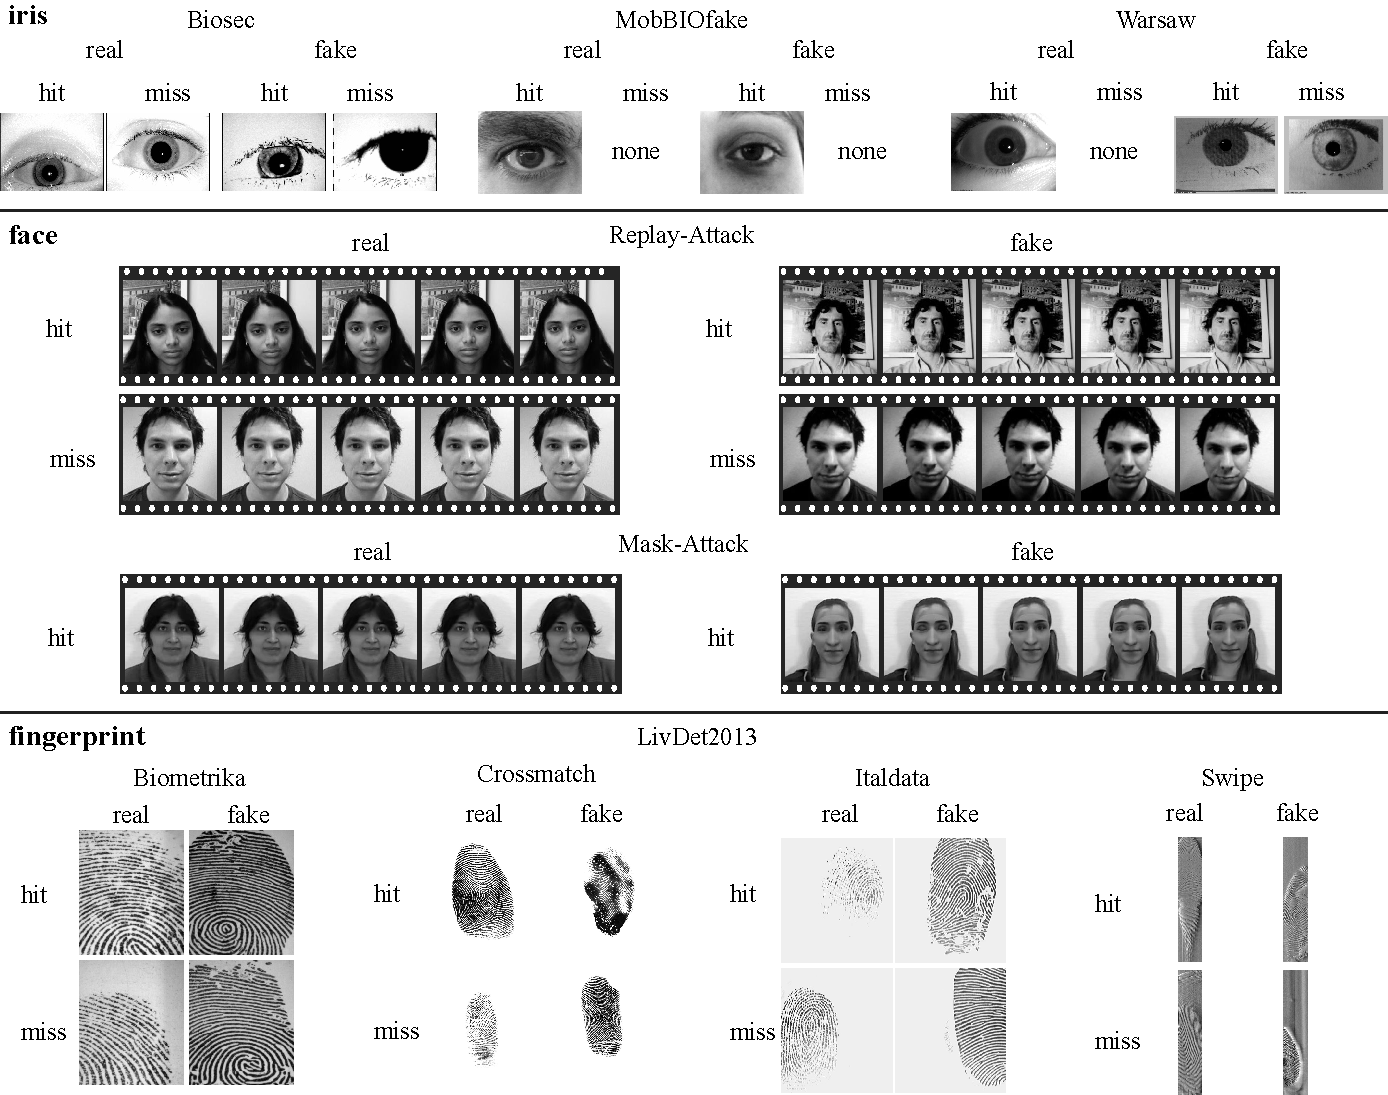
\includegraphics[width=0.85\linewidth]{datasets.pdf}
\caption{Examples of hit and missed testing samples lying closest to the real-fake decision boundary of each benchmark. A magnified visual inspection on these images may suggest some properties of the problem to which the learned representations are sensitive.}
\label{fig:datasets}\label{page:fig:datasets}
\end{center}
\end{figure*}


\subsection{Visual Assessment}

In Fig.~\ref{fig:datasets}, we show examples of hit and missed testing samples lying closest to the real-fake decision boundary of the best performing system in each benchmark. 
A magnified visual inspection on these images may give us some hint about properties of the problem to which the learned representations are sensitive.

While it is difficulty to infer anything concrete, it is interesting to see that the real missed sample in Biosec is quite bright, and that skin texture is almost absent in this case. 
% In contrast, we have achieved perfection classification for MobBIOfake database.
%Still, we may argue that a possible reason for the fake miss in MobBIOfake is the use of glasses, 
Still, we may argue that a noticeable difference exists in Warsaw between the resolution used to print the images that led to the fake hit and the fake miss.

Regarding the face benchmarks, the only noticeable observation from Replay-Attack is that the same person is missed both when providing to the system a real and a fake biometric reading. This may indicate that some individuals are more likely to successfully attack a face recognition systems than others. In 3DMAD, it is easy to see the difference between the real and fake hits. Notice that there was no misses in this benchmark.

A similar visual inspection is much harder in the fingerprint benchmarks, even though the learned deep representations could effectively characterize these problems. The only observation possible to be made here is related to the fake hit on CrossMatch, which is clearly abnormal.
The images captured with the Swipe sensor are naturally narrow and distorted due to the process of acquisition, and this distortion prevents any such observation.